\documentclass[listof=numbered,12pt,a4paper]{scrartcl}
\usepackage[scaled]{helvet}
\usepackage[T1]{fontenc}
\usepackage[utf8x]{inputenc}
\usepackage[ngerman]{babel}
\usepackage{geometry}
\usepackage{setspace}
\usepackage[printonlyused, withpage]{acronym}
\usepackage{graphicx}
\usepackage{graphics}
\usepackage{capt-of}
\usepackage[absolute]{textpos}
\usepackage[automark]{scrpage2}
\usepackage[procnames]{listings}
\usepackage{color}
\usepackage{url}
\usepackage{pdfpages}
\usepackage{hyperref}
% zwei Bilder nebeneinander darstellen
\usepackage{subfigure}
%\usepackage{titlesec}
%smiley-Packet
\usepackage{tikzsymbols}
\setkomafont{sectioning}{\bfseries} 
\setcounter{tocdepth}{5}
\setcounter{secnumdepth}{5}
\geometry{a4paper,left=30mm,right=20mm}
% beheben ds tightlist-Errors
\def\tightlist{}



% Nach \title{}
\DeclareFixedFont{\ttb}{T1}{txtt}{bx}{n}{12} % for bold
\DeclareFixedFont{\ttm}{T1}{txtt}{m}{n}{12}  % for normal
% Custom colors
\definecolor{deepblue}{rgb}{0,0,0.5}
\definecolor{deepred}{rgb}{0.6,0,0}
\definecolor{deepgreen}{rgb}{0,0.5,0}

\usepackage{listings}

% Python style for highlighting
\newcommand\pythonstyle{\lstset{
language=Python,
basicstyle=\ttm,
otherkeywords={self},             % Add keywords here
keywordstyle=\ttb\color{deepblue},
emph={MyClass,__init__},          % Custom highlighting
emphstyle=\ttb\color{deepred},    % Custom highlighting style
stringstyle=\color{deepgreen},
frame=tb,                         % Any extra options here
showstringspaces=false            %   
}}


% Python environment
\lstnewenvironment{python}[1][]
{
\pythonstyle
\lstset{#1}
}
{}

% Python for external files
\newcommand\pythonexternal[2][]{{
\pythonstyle
\lstinputlisting[#1]{#2}}}

% Python for inline
\newcommand\pythoninline[1]{{\pythonstyle\lstinline!#1!}}

% \code{TEXT} um TEXT als monospace (courier new) dazustellen
\newcommand{\code}[1]{\texttt{#1}}


\newcommand{\twopicinsert}[7] {
%\twopicinsert{weite1}{dateiname1 (ohne png)}{Abbildungbeschriftung1}{weite2}{dateiname2}{Abbildungbeschriftung2}{Gesamtbeschrift}}}
  \begin{figure}[h]
  \subfigure[#3]{\includegraphics[width=#1\textwidth]{./res/#2.png}}
  \subfigure[#6]{\includegraphics[width=#4\textwidth]{./res/#5.png}} 
  \caption{#7\label{fig:#3}} 
  \end{figure}
}


\newcommand{\picinsert}[3] {
% \picinsert{0.5}{dateiname (ohne png)}{Abbildungbeschriftung}
  \begin{figure}[h]
  \centering
  \includegraphics[width=#1\textwidth]{./res/#2.png}
% Bildtitel zur Referenzierung
  \caption{#3\label{fig:#2}}
  \end{figure}
}


\usepackage{graphicx}
% Redefine \includegraphics so that, unless explicit options are
% given, the image width will not exceed the width of the page.
% Images get their normal width if they fit onto the page, but
% are scaled down if they would overflow the margins.
\makeatletter
\def\ScaleIfNeeded{%
  \ifdim\Gin@nat@width>\linewidth
    \linewidth
  \else
    \Gin@nat@width
  \fi
}
\makeatother
\let\Oldincludegraphics\includegraphics
{%
 \catcode`\@=11\relax%
 \gdef\includegraphics{\@ifnextchar[{\Oldincludegraphics}{\Oldincludegraphics[width=\ScaleIfNeeded]}}%
}





% HIER: Autoren eintragen
\author{Vorname1 Nachname1 Vorname2 Nachname2 Vorname3 Nachname3}
\date{\today}
\title{Dokumentation}

\begin{document}
\parindent 0pt
\normalsize
\begin{titlepage}

\begin{center}


% Oberer Teil der Titelseite:  

\textsc{\huge Projektdokumentation}\\[1.5cm]

%{\huge Thema:}\\[0.5cm]


% Title
\newcommand{\HRule}{\rule{\linewidth}{0.5mm}}
\HRule \\[0.4cm]
{ \huge \bfseries Hier kommt ein ganz langer und ausführlicher Titel der Projektarbeit hin}\\[0.4cm]

\HRule \\[1.5cm]

% Author
\begin{minipage}{0.4\textwidth}
\begin{flushleft} \large
\emph{Autoren:}\\
% HIER: Autoren eintragen
Vorname1 Nachname1\\Vorname2 Nachname2\\Vorname3 Nachname3
\end{flushleft}
\end{minipage}
\par\bigskip
\par\bigskip
\begin{minipage}{0.4\textwidth}
\begin{flushleft} \large
\emph{Betreuer:}\\
Herr V. Nachname1\\Herr V. Nachname2
\end{flushleft}
\end{minipage}
\par\bigskip
\par\bigskip
\begin{minipage}{0.4\textwidth}
\begin{flushleft} \large
\emph{Abgabedatum:}\\
23. Mai 2018
\end{flushleft}
\end{minipage}
\par\bigskip
\par\bigskip
\begin{minipage}{0.4\textwidth}
\begin{flushleft} \large
\emph{Ort:}\\
Frankfurt am Main
\end{flushleft}
\end{minipage}
\par\bigskip
\par\bigskip
\begin{minipage}{0.4\textwidth}
\begin{flushleft} \large
\emph{Institution:}\\
Werner-von-Siemens-Schule
\end{flushleft}
\end{minipage}
\par\bigskip
\par\bigskip
\begin{minipage}{0.4\textwidth}
\begin{flushleft} \large
\emph{Zeitraum:}\\
September 2013 bis Mai 2014
\end{flushleft}
\end{minipage}
%\par\bigskip
%\par\bigskip
%\par\bigskip
%\begin{minipage}{0.4\textwidth}
%\begin{flushleft} \large
%\emph{Datum:}\\
%{\large \today}
%\end{flushleft}
%\end{minipage}
%{\large \today}
\end{center}

\end{titlepage}

\onehalfspacing
\pagenumbering{Roman}
\tableofcontents
\newpage
\pagestyle{scrheadings}
\clearscrheadfoot
\ihead[]{\bfseries\headmark}

% Überschrift vor Projekttitel
\ohead[]{Projektdokumentation}
% HIER: Fusszeile Namen anpassen
\ifoot[]{V. Nachname}
\ofoot[]{\pagemark}
\setheadsepline[\textwidth]{1pt}
\setfootsepline[\textwidth]{1pt}
\pagenumbering{arabic}


% Einleitung einbinden
\section{Einleitung}
\subsection{Vorwort}
Hier kommt ein nettes Vorwort hin. 

Neue Absätze werden durch zwei 'returns' eingefügt.

\subsection{Projektbeschreibung}
Natürlich sollte das Projekt kurz beschrieben werden. Das könnte man an dieser Stelle tun. Dieser Text sollte 
aber nicht zu lang werden, sonst bleibt nichts mehr für die eigentliche Dokumentation.


\par\bigskip
Den Befehl \code{\textbackslash par\textbackslash bigskip} kann man verwenden, wenn man einen größeren Abstand zwischen den Absätzen haben
möchte. Dies sollte aber nur in Ausnahmen genutzt werden, da sonst das Schriftbild darunter leidet.

Vielleicht kommen an dieser Stelle auch schon die ersten Abkürzungen wie \ac{LDAP}.

\subsection{Aufgabenverteilung}
Die Aufgaben der einzelnen Projektmitglieder sollten klar benannt werden.
Dies könnte hier geschehen.
\begin{itemize}
\item Projektteil 1 blablabla
\item Projektteil 2 blablabla
\item Projektteil 3 blablabla
\end{itemize}

Und schon ist unsere Einleitung fertig. \Winkey


% Projektumgebung einbinden
\newpage
\section{Projektumgebung}
Im Kapitel Projektumgebung kann der Umfeld in dem das Projekt stattfand beschrieben werden. 
Hier können natürich wieder einige Unterkapitel kommen. Diese werden mit dem Befehl 
\code{\textbackslash subsection\{Unterkapiteltext\}} eingefügt.

\subsection{Unterkapitel zur Projektumgebung}
Eventuell kommt man mit einem Unterkapitel nicht aus. Kein Problem dann fügt man eben noch weitere hinzu.

\subsubsection{Und noch ein Unterkapitel zur Projektumgebung}
bla bla bla

\subsubsection{Soviele Unterkapitel zur Projektumgebung}
bla bla bla

\textbf{Extrabereich1}$\;$\\
Wenn man mal etwas fett aber ohne eigene Überschrift verwenden möchte.

\newpage
\textbf{Extrabereich2}$\;$\\
Und noch etwas vervorgehobenes
Das folgende Bild wurde durch ein neues Kommando eingefügt:
\code{\textbackslash picinsert\{0.5\}\{hyperbel\_kreis\_ellipse\}\{Hyperbel mit Kreis\}}
Dabei werden die Parameter in \{\}

\picinsert{0.5}{hyperbel_kreis_ellipse}{Hyperbel mit Kreis}





\subsubsection{Aufzählungen und wie man sie anlegt}
Eine tolle Sache sind auch Aufzählungen. Diese können per \code{\textbackslash begin\{itemize\}} eingeleitet.
Die einzelnen Punkte werden dann mit \code{\textbackslash item} Zeile für Zeile eingefügt.
Wo ein \code{begin} ist gibt es natürlich auch ein \code{end}.
\begin{itemize}
\item Punkt 1
\item Punkt 2 
\item Punkt 3
\end{itemize}


% Allgemeine Zielsetzung des Projekts einbinden
\subsection{Unterkapitel mit einer weiteren Zielsetzung}
\subsubsection{Unterkapitel dazu}

Dann haben wir die Zielsetzungen für alle Teilnehmer definiert. Puh...


% Realisierung 
\newpage
\section{Durchführung}
\subsection{Mal fremde ``Federn'' einfügen}
So könnt man einen fremden Text zitieren:
\begin{quote}
``Hier steht der fremde Text der zitiert werden soll. bla bla bla ''
\newline
\url{https://de.wikipedia.org/wiki/Projekt} 20.05.2014 18:48 Uhr
\end{quote}
\subsubsection{Und noch ein Kapitel}
\paragraph{Wir kommen mit den Ebenen nicht aus}$\;$\\
bla bla bla 
\paragraph{Relative Distinguished Name}$\;$\\
Und hier noch ein Literaturverweis auf [Scheibner2011]
bla bla bla 

Wenn man Sourcecode schreibt soll dieser natürlich gut aussehen in der Dokumentation. Dies kann man z.B. so 
darstellen wie hier:
\begin{python}
dn: dc=schule, ou=People,uid=ti2a
objectClass: account
uidNumber: 2000
description: 2015
\end{python}

Die Darstellung hilft zur Strukturierung des Textes und gibt Übersicht.
\begin{python}
import ldap
\end{python}

\begin{python}
return template('static/pwneusetzen.tpl', user = user, 
			fehler = '', success = 'true',
			liste = liste1)
else:
	return template('static/pwneusetzen.tpl', 
	user = user, fehler = 'true', 
	success = '', liste = liste1)
\end{python}

Manchmal möchte man aber nicht einen ganzen Abschnitt als Code darstellen, sondern nur ein paar Befehle 
innerhalb des Textes \code{\textbackslash pythoninline} hilft dabei einen Befehl wie \pythoninline{command} 
entsprechend darzustellen.

Quellcode im Python-Skript:
\begin{python}
if inputcheck(uid, password) == True:
	if syntaxchecken(uid) == True:
		if userexsits(uid) == False:
\end{python}




% Zusammenfassung einbinden
\section{Zusammenfassung Teil 1}
War das nicht alles schön hier...

Der Rest der Zusammenfassung kommt noch.


% Ende des Haupttextes einbinden inkl. Unterschriften usw.
\newpage
\section{Ausblick}
Falls man noch etwas für die Zukunft mitgeben möchte könnte man das hier tun. Oder auch lassen \Winkey
\twopicinsert{0.5}{hyperbel_kreis_ellipse}{Hyperbel mit Kreis}{0.5}{hyperbel_parabel_hyperbel}{Hyperbel mit Parabel}{Überschrift für beide Bilder}

\newpage
Der folgende Teil ist wichtig und sollte auf jeden Fall enthalten sein.

\section{Eigenständigkeitserklärung}
Ich versichere hiermit, dass ich die vorliegende Projektdokumentation mit dem Thema 
\begin{quote}
``Entwicklung einer Web-Oberfläche zur Verwaltung eines LDAP-Servers sowie zur Verteilung von Images über ein lokales Netzwerk''
\end{quote}
 selbständig verfasst und keine anderen als die angegebenen Quellen und Hilfsmittel benutzt habe. Alle wörtlich und sinngemäß aus veröffentlichten oder nicht veröffentlichten Schriften entnommenen Stellen sind als solche kenntlich gemacht.

Weiterhin erkläre ich, dass die Arbeit in gleicher oder ähnlicher Form noch keiner anderen Prüfungsbehörde vorgelegen hat und noch nicht veröffentlicht wurde.

\vspace{1.5cm}
\begin{tabular}{lp{2em}l}
 \hspace{6cm}   && \hspace{6cm} \\\cline{1-1}\cline{3-3}
 Ort, Datum     && Unterschrift
\end{tabular}
\par\bigskip
\vspace{1.5cm}
\begin{tabular}{lp{2em}l}
 \hspace{6cm}   && \hspace{6cm} \\\cline{1-1}\cline{3-3}
 Ort, Datum     && Unterschrift
\end{tabular}
\par\bigskip
\vspace{1.5cm}
\begin{tabular}{lp{2em}l}
 \hspace{6cm}   && \hspace{6cm} \\\cline{1-1}\cline{3-3}
 Ort, Datum     && Unterschrift
\end{tabular}



% Abkürzungsverzeichnis einbinden
\newpage
%Abkürzungsverzeichnis
% wird in Main-Dokument eingebunden SICH HIER IM MAIN DOKUMENT
%\acro{Abkürzung}{Ausgeschrieben} -> Neue Abkürzung anlegen
% IM TEXT \ac{Abkürzung} -> Gibt EINMAL vollen Text mit Abkürzung in Klammern, danach %nur noch Abkürzung an
% Beispiel: \ac{cloop}
\section{Abkürzungsverzeichnis}
\begin{acronym}[Bash]
\acro{cloop}{compressed loop device}
\acro{cpu}{change passwort utility}
\acro{CSS}{Cascading Style Sheets}
\acro{DN}{Distinguished Name}
\acro{HTML}{Hypertext Markup Language}
\acro{KVM}{Kernel-based Virtual Machine}
\acro{LDAP}{Lightweight Directory Access Protocol}
\acro{LDIF}{LDAP data interchange format}
\acro{Linbo}{Linux-based Network Boot Operating System}
\acro{LTS}{Long Term Support}
\acro{NIS}{Network Information Service}
\acro{OS}{Operating System}
\acro{PXE}{Preboot Execution Environment}
\acro{RDN}{Relative Distinguished Name}
\acro{SheilA}{Selbstheilende Arbeitsstation}
\acro{SSH}{Secure Shell}
\acro{ul}{Unordered List}
\acro{li}{List Item}
\acro{ol}{Ordered List}
\acro{URI}{Uniform Resource Identifier}
\acro{VM}{virtuelle Maschine}
\acro{W3C}{World Wide Web Consortium}
\end{acronym}
\newpage


% Abbildungsverzeichnis einbinden
\listoffigures

% Literaturverzeichnis einbinden
\newpage
\section{Literatur}
[Barry2011] Barry, Paul (2011): Python von Kopf bis Fuß
\newline
\par\smallskip
[Scheibner2011][PDF] Scheibner, Alexander (2011): LDAP - Verzeichnisdienst nicht nur für Unix. Version 0.91, Seitenzahl 49, Datum der Sicherung 04.07.2013
\newline
\par\smallskip
[Weigend2013] Weigend, Michael (2013): Python GE-PACKT. 5. Auflage
\newline
\par\smallskip
[Robson; Freeman 2012] Robson, Elisabeth \& Freemann, Eric (2012): HTML und CSS von Kopf bis Fuß. 2. Auflage. O'Reilly Verlag GmbH \& Co. KG




% Anhang einbinden
\newpage
\section{Anhang}
\subsection*{Beispiel für als PDF eingefügte Bilder}

Die Unterüberschrift wurde ohne Nummerierung eingefügt. Dies wurde durch ein ``*'' hinter dem \code{subsection} Befehl erreicht.

Man kann auch gleich ganze PDF-Dokument einfügen. Viel Spaß damit bei anderen Programmen. \Winkey
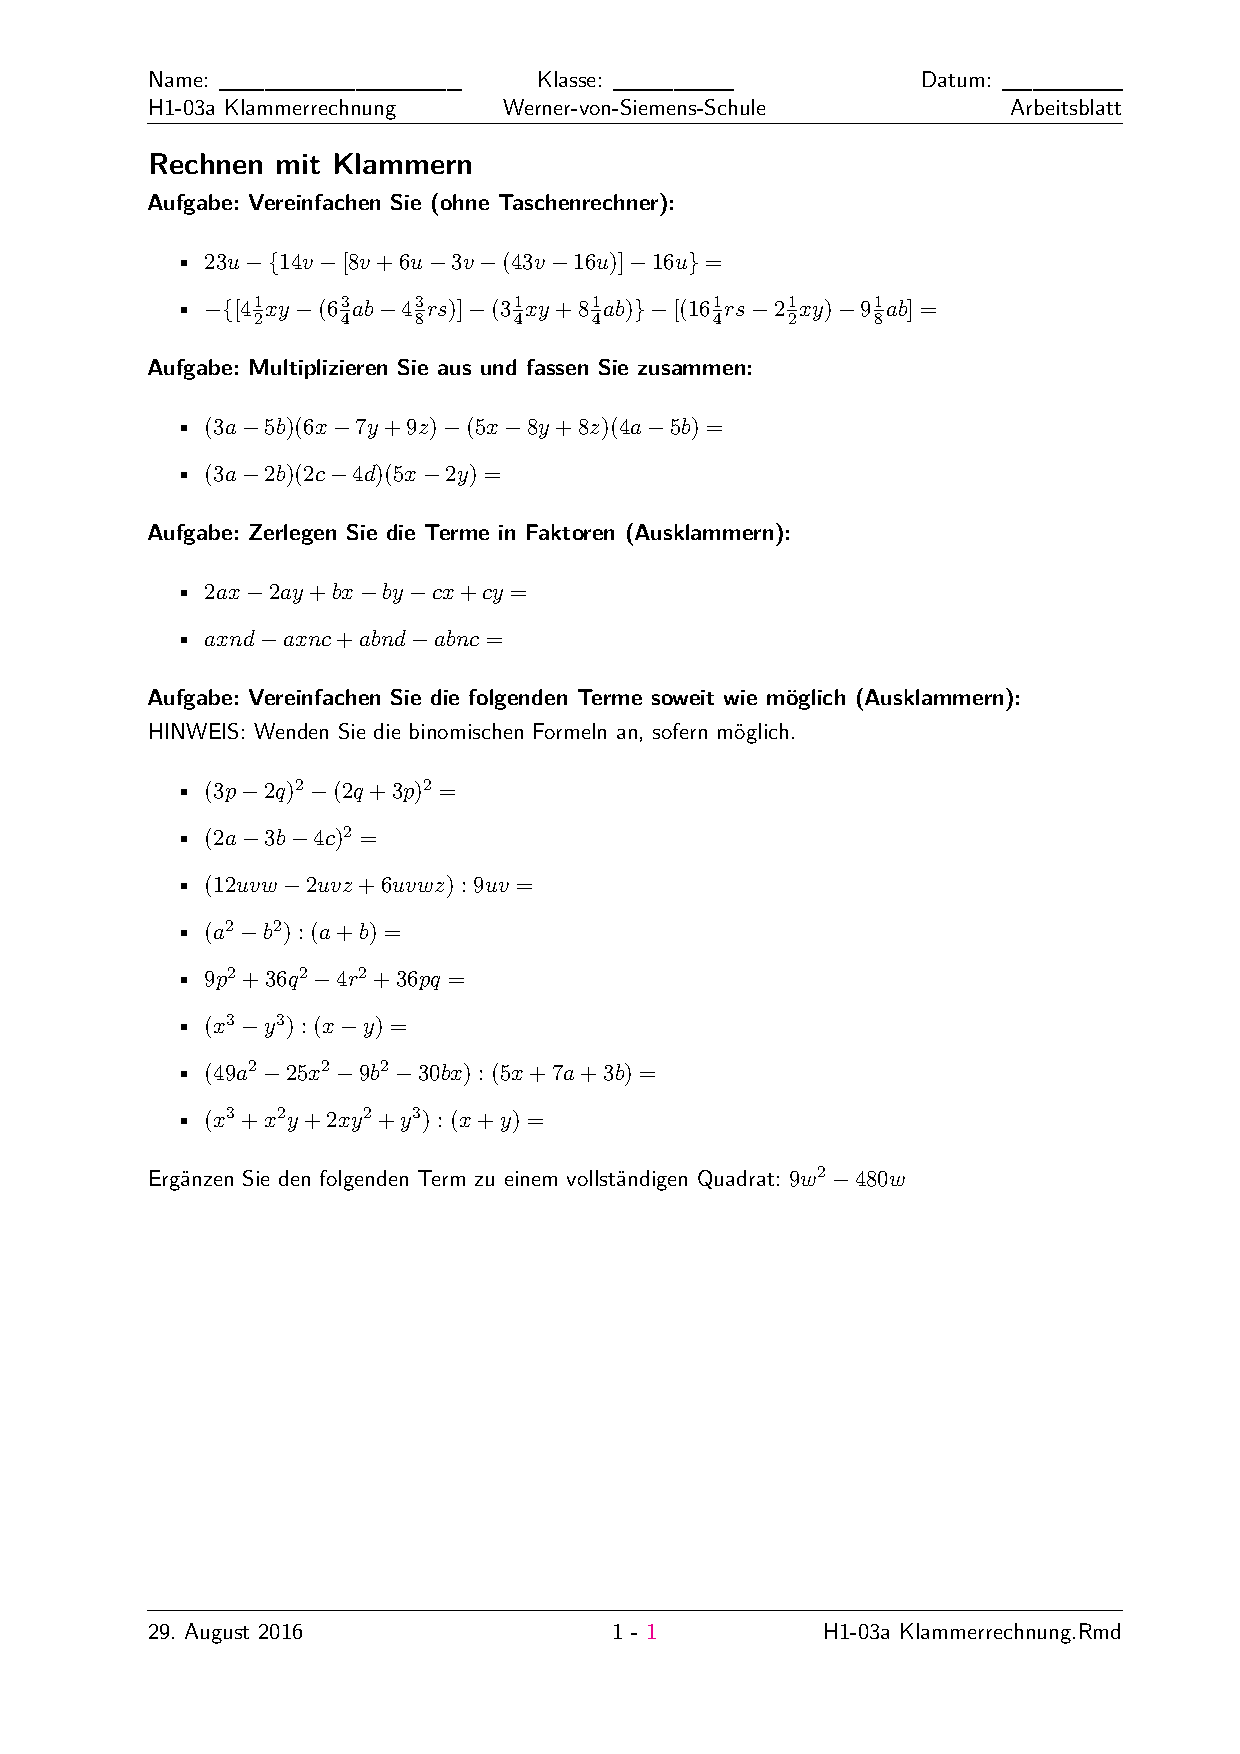
\includepdf[landscape]{./res/klammerrechnung.pdf}

\end{document}
